

\section{Courbes paramétrées}

\subsection{Terminologie des courbes paramétrées en dimension $3$}

\begin{Def} \textbf{Courbe paramétrée}

Une courbe paramétrée est une fonction vectorielle (de classe \( C^1 \))
\[
\gamma : 
\begin{array}{ccc}
[a, b]& \to &\mathbb{R}^3 \\
t& \mapsto &\big(x(t), y(t), z(t)\big)
\end{array}
\]

Le \textbf{support} de la courbe paramétrée est le lieu des points
\[
C = \Big\{ \gamma(t) = \big(x(t), y(t), z(t)\big), \, t \in [a, b]  \Big\}\,.
\]
\end{Def}

\begin{Rmq}
On étend la définition des courbes paramétrées aux courbes de classe \( C^1 \) par morceaux : on
dit que \(\gamma\) est de classe \( C^1 \) par morceaux si \(\gamma\) est continue sur \( I = [a, b] \) et on peut subdiviser l'intervalle \( I \) en
un nombre fini de sous-intervalles \( a = a_0 < a_1 < \cdots < a_n = b \) tel que la restriction de \(\gamma\) à \([a_i, a_{i+1}]\) soit de
classe \( C^1 \) pour tout \( 0 \leq i \leq n - 1 \).

\begin{itemize}
    \item Le point \(\gamma(a)\) (resp. \(\gamma(b)\)) est appelé l'origine (resp. l'extrémité) du chemin \(\gamma\).
    \item On dit qu'un chemin \(\gamma\) est contenu dans un sous-ensemble \( D \) de \( \mathbb{R}^3 \), si son support \( C \subset D \).
    \item Une courbe paramétrée est naturellement orientée par le sens croissant du paramètre \( t \). On note dans ce
    cas le support par \( C^+ \) et on dit qu'il est orienté dans le sens direct (ou positif).
    \item Le support de \(\gamma\) parcouru dans le sens inverse (ou négatif) est noté \( C^- \), il est par exemple paramétré
    par \(\tilde{\gamma} : [a, b] \to \mathbb{R}^3 \) définie par \(\tilde{\gamma}(t) = \gamma(a + b - t)\).
    \item On dit que la courbe \(\gamma\) est fermée quand \( I = [a, b] \) et \(\gamma(a) = \gamma(b)\).
    \item On dit qu'une courbe \(\gamma\) est simple si \(\gamma(t) \neq \gamma(t_0)\), pour tout \( t, t_0 \in ]a, b[ \) tels que \( t \neq t_0 \), i.e. \(\gamma\) sur \(|]a,b[ \) est injective.
\end{itemize}
\end{Rmq}


\begin{Def} \textbf{Vecteur vitesse}

On appelle vecteur vitesse la dérivée première de \(\gamma\) :
\[
\gamma'(t) = \frac{d\gamma(t)}{dt} = \Big(x'(t), y'(t), z'(t)\Big)
\]
\end{Def}

\begin{Def}\textbf{Régularité}

Une courbe paramétrée \(\gamma : I \to \mathbb{R}^3\) est dite régulière si pour tout \(t \in I\), \(\|\gamma'(t)\| \neq 0\), autrement dit, si son vecteur vitesse ne s'annule jamais. La droite passant par \(\gamma(t)\) et de vecteur directeur \(\gamma'(t)\) est appelée la droite tangente en \(t\) à \(\gamma\).
\end{Def}

\begin{Def} \textbf{Longueur}

La longueur de la courbe paramétrée \(\gamma : I \to \mathbb{R}^3\) entre \(t_0\) et \(t_1\) (\(a \leq t_0 \leq t_1 \leq b\)) est donnée par
\[
L_{t_1}^{t_0}(\gamma) = \int_{t_0}^{t_1} \|\gamma'(t)\| \, dt = \int_{t_0}^{t_1} \sqrt{(x'(t))^2 + (y'(t))^2 + (z'(t))^2} \, dt
\]


\end{Def}


\begin{Ex}
Soit \(\gamma(t) = (t, t, t)\) avec \(t \in [0, 1]\).\\
On a \(\gamma'(t) = (1, 1, 1)\) d'où \(\|\gamma'(t)\| = \sqrt{1 + 1 + 1} = \sqrt{3} \neq 0\).\\
Ainsi \(\gamma\) est régulière.\\


\end{Ex}


\begin{Ex} 
\begin{small}
Soit \(\gamma(t) = (3 \cos t, 0, 2 \sin t)\) avec \(t \in [0, 2\pi]\).\\
On a \(x(t)/3 = \cos t\), \(y(t) = 0\) et \(z(t)/2 = \sin t\),\\
ainsi le support de la courbe est l'ellipse contenue dans le plan \(\{y = 0\}\), d'équation \(\frac{x^2}{9} + \frac{z^2}{4} = 1\).\\
Puisque \(\gamma(t) = (3 \cos t, 0, 2 \sin t)\), on a \(\gamma'(t) = (-3 \sin t, 0, 2 \cos t)\) 

d'où \(\|\gamma'(t)\| = \sqrt{9 \sin^2 t + 4 \cos^2 t} \neq 0\).\\
Ainsi \(\gamma\) est régulière.
\end{small}
\end{Ex}

\begin{Ex}

\begin{small}
Soit \(\gamma(t) = (\cos t, \sin t, t)\) avec \(t \in [0, 6\pi]\).\\

On a \(x^2(t) + y^2(t) = 1\),\\ 
le support de la courbe est contenu dans un cylindre de base un cercle unité.\\
La hauteur \(z(t)\) est le paramètre angulaire. Le support de la courbe est donc une hélice.

Puisque \(\gamma(t) = (\cos t, \sin t, t)\), on a \(\gamma'(t) = (-\sin t, \cos t, 1)\) par suite \(\|\gamma'(t)\| = \sqrt{\sin^2 t + \cos^2 t + 1} = \sqrt{2}\),\\
ainsi la courbe \(\gamma\) est régulière.

La longueur de \(\gamma\) entre \(0\) et \(2\pi\) vaut
\[
L_{2\pi}^{0}(\gamma) = \int_{0}^{2\pi} \sqrt{2} \, dt = 2\sqrt{2}\pi.
\]
\end{small}

\end{Ex}
\subsection{Terminologie des courbes paramétrées en dimension $2$}

\begin{Def}\textbf{Courbe paramétrée}\\
On appelle \textbf{courbe paramétrée (ou arc paramétré)} la donnée d'une application $\phi : A \to P$ où $A$ est une partie de $\R$ et $P$ le plan des points.\\
 On appelle support ou trajectoire de la courbe l'ensemble des
points atteints par le mouvement : $$C = \{ M \in P | \exists t \in A, M = \phi(t) \} =\hat{\phi}(A).$$
\end{Def}
\begin{Rmq}
\begin{itemize}\item  Si le plan est rapporté à un repère cartésien $\mathcal{R} = (O, \overrightarrow{i} ,\overrightarrow{j} )$, ceci revient à donner deux fonctions
$x : A  \longrightarrow  \R$ et $y : A  \longrightarrow  \R$ telles que : $$\forall t \in A, \phi(t) = (x(t), y(t))_\mathcal{R}.$$
 Cela revient aussi à donner une fonction vectorielle $\vec{f} : A  \longrightarrow  P$ telle que :
$ \forall t  \in  A,  \vec{f} (t) = \vec{ O\phi(t)}$.\\
 On note $M_t = \phi(t)$ ; $\vec{f} (t) = \vec{OM_t}$.\\
\item Une courbe paramétrée n'est pas qu'une courbe du plan, il y a aussi une idée de mouvement, donc de vitesse, de sens de parcours, d'accélération : c'est de la dynamique.\\
\item On peut définir une même courbe en cartésiennes, en polaires, par une fonction numérique.\\
\end{itemize}



\end{Rmq}


\begin{Ex}

 Le demi-cercle de centre $O$ et de rayon $1$ privé des points $(1, 0)_\mathcal{R}$ et $(-1, 0)_\mathcal{R}$\\
 (en supposant $\mathcal{R}$ orthonormé direct) peut être donné par\\
 $x(	\theta) = \cos(\theta)$ et $y(	\theta) = \sin(\theta)$ (en cartésiennes)\\
 
mais aussi par $\rho(	\theta) = 1$ (en polaires) pour $\theta \in ]0, \pi[$ ou par $x_1(t) = \dfrac{1 - t^2}{ 1 + t^2}$ et\\
$y_1(t) =\dfrac{ 2t}{1 + t^2}$ (en cartésiennes) pour $t \in]0, +\infty[$ \\

et même par $y(x) = \sqrt{1 - x^2}$ (fonction) pour$ x  \in ] - 1, 1[$.\\

\end{Ex}


\subsection{Limite et dérivée d'une fonction vectorielle de la variable réelle}
\begin{Def}\textbf{Limite d'une fonction vectorielle}\\

Soit $\vec{f} : A \to P$ une fonction vectorielle de la variable réelle.\\
 Si $a \in A$ et $\vec{v} \in P$, on dira que $\vec{f}$ admet pour limite $\vec{v}$ en $a$ qu'on écrira $$\lim_{t \to a} \vec{f}(t) = \vec{v}\text{ si }\lim_{t \to a} ||\vec{f}(t) - \vec{v}|| = 0.$$
\end{Def}

\begin{Rmq} 
\begin{itemize}
    \item Avec ces notations, si on note \\
    $\vec{f}(t) = \begin{pmatrix} x(t) \\ y(t) \end{pmatrix}_B$ et $\vec{v} = \begin{pmatrix} v_1 \\ v_2 \end{pmatrix}_B$ les coordonnées dans une base orthonormée $B$, alors\\
    $\lim_{t \to a} \vec{f}(t) = \vec{v} \iff \left( \lim_{t \to a} x(t) = v_1 \text{ et } \lim_{t \to a} y(t) = v_2 \right)$.
    \item On peut aussi définir la dérivée d'une fonction vectorielle et on a un résultat similaire qui dit que $\vec{f}$ est dérivable en $a$ ssi les fonctions coordonnées $x$ et $y$ le sont et qu'on a alors : $\vec{f}'(a) = \begin{pmatrix} x'(a) \\ y'(a) \end{pmatrix}_B$.
\end{itemize}
\end{Rmq}

\begin{Prop}\textbf{Dérivées de fonctions vectorielles}\\
Soit $\vec{f}$ et $\vec{g}$ deux fonctions vectorielles dérivables sur $A$, alors $\vec{f} \cdot \vec{g}$, $||\vec{f}||$ (si $\vec{f}$ ne s'annule pas sur $A$) %et $\det(\vec{f}, \vec{g})$
 le sont aussi sur $A$.
\begin{align*}
    (\vec{f} \cdot \vec{g})' &= \vec{f}' \cdot \vec{g} + \vec{f} \cdot \vec{g}', \\
    ||\vec{f}||' &= \frac{\vec{f} \cdot \vec{f}'}{||\vec{f}||}, \\
    %\det(\vec{f}, \vec{g})' &= \det(\vec{f}', \vec{g}) + \det(\vec{f}, \vec{g}').
\end{align*}
\end{Prop}

\subsection{Point stationnaire, point régulier, tangentes}

On note $M_t = \varphi(t)$ un point de la courbe et $\overrightarrow{f}(t) = \overrightarrow{OM_t}$ le vecteur entre l'origine du repère orthonormé direct $\mathcal{R}$ et le point $M_t$ de la courbe.


\begin{Def}\textbf{Point stationnaire, point régulier, tangentes}\\
On suppose dans les définitions suivantes que la courbe est "assez" dérivable :\\

\begin{itemize}
    \item On dit que $M_{t_0}$ $(t_0 \in A)$ est un \textbf{point régulier} si $\overrightarrow{f}'(t_0) \neq \overrightarrow{0}$.
    \item On dit que $M_{t_0}$ est un point \textbf{stationnaire} s'il n'est pas régulier.
    \item On dit que la courbe est régulière si tout point de la courbe est régulier.
    \item On dit que le point $M_{t_0}$ est un point \textbf{birégulier} si $\overrightarrow{f}'(t_0)$ et $\overrightarrow{f}''(t_0)$ ne sont pas colinéaires.
    \item On dit que la courbe est birégulière si tout point de la courbe est birégulier.\\
\end{itemize}

\end{Def}

\begin{Rmq}
En un point régulier $M_{t_0}$, si $t \in A$ et $t \neq t_0$ et $M_t \neq M_{t_0}$ alors le vecteur $\overrightarrow{M_{t_0}M_t} / (t - t_0)$ est un vecteur directeur de la droite $(M_t M_{t_0})$. Ce vecteur a pour vecteur limite la dérivée $\overrightarrow{f}'(t_0)$ qui oriente donc la tangente à la courbe en $M_{t_0}$.\\
\end{Rmq}
\begin{Prop}\textbf{Tangente}\\

    La tangente à la courbe en un point régulier $M_{t_0}$ a  pour équation cartésienne :
\[
\frac{x - x(t_0)}{x'(t_0)} - \frac{y - y(t_0)}{y'(t_0)} = 0.
\]
\end{Prop}


\begin{Rmq}
\begin{itemize}
    \item En un point stationnaire $M_{t_0}$, on pourra tout de même avoir une équation de la tangente en calculant $\frac{y(t) - y(t_0)}{x(t) - x(t_0)}$ : cela donnera la pente de la tangente en $M_{t_0}$ à la courbe.
    \item Le mouvement est dit \textbf{rectiligne} s'il existe une droite $D$ telle que : $\forall t \in A, M_t \in D$.
    \item Le mouvement est dit à \textbf{accélération centrale} si : $\exists C \in P, \forall t \in A, \overrightarrow{f}''(t)$ et $\overrightarrow{CM_t}$ sont colinéaires.\\
\end{itemize}
\end{Rmq}

\begin{Rmq}
On se place au voisinage d'un point $M_{t_0}$, on suppose la fonction $\overrightarrow{f}$ suffisamment dérivable pour pouvoir définir $p > 1$ le plus petit entier tel que la dérivée $\overrightarrow{f}^{(p)}(t_0) \neq \overrightarrow{0}$ et $q > p$ le plus petit entier tel que $\overrightarrow{f}^{(p)}(t_0)$ et $\overrightarrow{f}^{(q)}(t_0)$ ne sont pas colinéaires.\\
 En appelant $(X, Y)$ les coordonnées de $M_{t_0+h}$ dans le repère $(M_{t_0}, \overrightarrow{f}^{(p)}(t_0), \overrightarrow{f}^{(q)}(t_0))$, on a :
\[
\begin{cases}
X \underset{0}{=} \alpha h^p (1 + \cdots) + \beta h^q + o(h^q) \\
Y \underset{0}{=} \gamma h^q + o(h^q)
\end{cases}
\]



Ainsi, on a 4 cas à considérer pour l'allure locale de la courbe au voisinage de $M_{t_0}$ :
\begin{itemize}
    \item Si $p$ est impair et $q$ est pair, $M_{t_0}$ est un point à \textbf{allure normale} (la courbe traverse localement toutes les droites passant par $M_{t_0}$ sauf la tangente).
    \item Si $p$ est impair et $q$ est impair, $M_{t_0}$ est un \textbf{point d'inflexion} (la courbe traverse localement toutes les droites passant par $M_{t_0}$).
    \item Si $p$ est pair et $q$ est impair, $M_{t_0}$ est un \textbf{point de rebroussement de première espèce} (la courbe ne traverse localement aucune droite passant par $M_{t_0}$ sauf la tangente).
    \item Si $p$ est pair et $q$ est pair, $M_{t_0}$ est un \textbf{point de rebroussement de seconde espèce} (la courbe ne traverse localement aucune droite passant par $M_{t_0}$).\\
\end{itemize}
\end{Rmq}


\begin{Rmq}


Pour une courbe donnée en coordonnées cartésiennes par \( M_t = \begin{pmatrix} x(t), y(t) \end{pmatrix}_R \), les expressions des dérivées première et seconde sont :

\[
\vec{f}'(t) = \begin{pmatrix} x'(t), y'(t) \end{pmatrix}_B
\]

et

\[
\vec{f}''(t) = \begin{pmatrix} x''(t), y''(t) \end{pmatrix}_B.
\]

Pour une courbe donnée en coordonnées polaires par \( \rho = \rho(\theta) \), c'est-à-dire par \( \vec{f}(\theta) = \rho(\theta)\vec{u}_{\theta} \), on a :

\[
\vec{u}_{\theta} = \begin{pmatrix} \cos(\theta) \\ \sin(\theta) \end{pmatrix}_B \quad \text{et} \quad \vec{v}_{\theta} = \begin{pmatrix} -\sin(\theta) \\ \cos(\theta) \end{pmatrix}_B
\]

Sachant que \( \vec{u}_{\theta}' = \vec{v}_{\theta} \) et \( \vec{v}_{\theta}' = -\vec{u}_{\theta} \), on peut écrire les expressions des dérivées première et seconde de \( \vec{f}(\theta) \) :

\[
\vec{f}'(\theta) = \rho'(\theta) \vec{u}_{\theta} + \rho(\theta) \vec{v}_{\theta}
\]

et

\[
\vec{f}''(\theta) = \left( \rho''(\theta) - \rho(\theta) \right) \vec{u}_{\theta} + 2\rho'(\theta) \vec{v}_{\theta}.
\]



\end{Rmq}
\section{Courbes en cartésiennes}

On se donne donc dans cette partie une courbe paramétrée en coordonnées cartésiennes (il est sous-entendu que le repère considéré est le repère canonique donc orthonormé direct) par :
\[
\begin{cases}
x = x(t) \\
y = y(t)
\end{cases}
\]

\subsection{Domaine d'étude et tableau de variations}

\begin{Meth}

\begin{enumerate}
  \item
 On détermine d'abord le domaine de définition $D_f$ de la courbe paramétrée qui est donc l'intersection des domaines de définition des fonctions $t \mapsto x(t)$ et $t \mapsto y(t)$.\\



\item On détermine ensuite le domaine d'étude :\\
 c'est-à-dire un domaine inclus dans le domaine de définition et qui permet, si on étudie correctement la courbe sur cette partie-là, de retrouver toute la courbe par des considérations de symétrie, de rotation, de translation, ...\\
 
 
 
\item On calcule les limites de $x$ et $y$ aux bornes de leurs domaines de définition. Si les fonctions $x$ et $y$ sont dérivables, on calcule ces dérivées là où elles existent et on fait l'étude du signe de ces dérivées pour connaître les variations de $x$ et de $y$. On dispose enfin toutes ces informations dans un tableau de variations qui se présente comme ceci :\\
\[ \left\{
\begin{array}{cl}


\text{1ère ligne} & \text{valeurs permises de } t \\

\text{2ème ligne} & \text{signe de } x'(t)  \\

\text{3ème ligne}  & \text{valeurs, variations, limites de } x(t)   \\

\text{4ème ligne} &   \text{valeurs, variations, limites de } y(t)  \\

\text{5ème ligne} &   \text{signe de } y'(t) \\

\end{array}
\right.
\]


\end{enumerate}

\end{Meth}



\begin{Ex}
Si on se donne une courbe paramétrée par $x(t) = \ln(t)$ et $y(t) = \sqrt{1 - t^2}$ \\
alors le domaine de définition est $\mathbb{R}^*_{+} \cap [-1; 1] = ]0; 1]$.\\
\end{Ex}

\begin{Rmq} 
\begin{itemize}
  \item Si $x$ et $y$ sont $T$-périodiques alors on peut étudier la courbe sur $D_f \cap \left[ -\frac{T}{2}, \frac{T}{2} \right]$ ou $Df \cap [0; T]$ et on repassera une infinité de fois par chacun des points de la courbe.\\
  \item Si $x$ et $y$ sont paires on peut étudier la courbe sur $D_f \cap \mathbb{R}^+$ et on repassera deux fois par chacun des points de la courbe.\\
  \item Si $x$ est paire et $y$ impaire alors on peut étudier et tracer la courbe sur $D_f \cap \mathbb{R}^+$ et on obtiendra ensuite toute la courbe par une symétrie d'axe $(Ox)$.\\
  \item Si $x$ est impaire et $y$ paire alors on peut étudier et tracer la courbe sur $D_f \cap \mathbb{R}^+$ et on obtiendra ensuite toute la courbe par une symétrie d'axe $(Oy)$.\\
  \item Si $x$ et $y$ sont impaires alors on peut étudier et tracer la courbe sur $D_f \cap \mathbb{R}^+$ et on obtiendra ensuite toute la courbe par une symétrie centrale autour de $O$.\\
\end{itemize}
\end{Rmq}



\begin{Ex}

 Si on veut étudier la cycloïde $x(t) = a(t - \sin t)$, $y(t) = a(1 - \cos t)$ (avec $a \in \mathbb{R}^*_+$),\\
 on voit que l'ensemble de définition est $\mathbb{R}$, on a\\
 $x(t + 2\pi) = x(t) + 2\pi a$ et $y(t + 2\pi) = y(t)$ donc\\
 on en déduit que la courbe est stable par la translation de vecteur $\overrightarrow{u}(2\pi a, 0)$ et\\
 on peut n'étudier que $[-\pi; \pi]$.\\
 De plus $x$ est impaire et $y$ est paire et\\
 on peut étudier sur $[0; \pi]$ et retrouver toute la courbe\\
 en faisant une symétrie orthogonale par rapport à la droite $(Oy)$.\\
\end{Ex}


\subsection{Branches infinies et point multiples}


\begin{Def}\textbf{Branches infinies}\\
On dit que la courbe paramétrée $f : I \rightarrow P$ présente une \textbf{branche infinie} lorsque $t$ tend vers $t_0$ si
\[
\lim_{t \to t_0} \| \overrightarrow{OM_t} \| = +\infty \quad (t_0^+, t_0^-, t_0 = +\infty \text{ et } t_0 = -\infty \text{ sont possibles}).
\]
On dit qu'une droite $D$ est asymptote à la courbe lorsque $t$ tend vers $t_0$ si 
\[
\lim_{t \to t_0} d(M_t, D) = 0.
\]

\end{Def}

\begin{Rmq}
\begin{itemize}
    \item Si $\lim_{t \to t_0} x(t) = \pm \infty$ et $\lim_{t \to t_0} y(t) = y_0$ alors la droite $y = y_0$ est asymptote à la courbe.\\
    De même, si $\lim_{t \to t_0} x(t) = x_0$ et $\lim_{t \to t_0} y(t) = \pm \infty$ alors $x = x_0$ est asymptote.\\
    \item Dans les autres cas, quand $x$ et $y$ tendent toutes les deux vers $\pm \infty$ quand $t$ tend vers $t_0$, on essaie d'estimer la quantité $\frac{y(t)}{x(t)}$ quand $t$ tend vers $t_0$. On a alors plusieurs cas :\\
    \begin{itemize}
        \item $\lim_{t \to t_0} \frac{y(t)}{x(t)} = \pm \infty$ : la courbe admet une branche parabolique de direction $(Oy)$ en $t_0$.\\
        \item $\lim_{t \to t_0} \frac{y(t)}{x(t)} = 0$ : la courbe admet une branche parabolique de direction $(Ox)$ en $t_0$.\\
        \item $\lim_{t \to t_0} \frac{y(t)}{x(t)} = a \in \mathbb{R}$ et $\lim_{t \to t_0} (y(t) - ax(t)) = \pm \infty$ : la courbe admet une branche parabolique de direction asymptotique $y = ax$ en $t_0$.\\
        \item $\lim_{t \to t_0} \frac{y(t)}{x(t)} = a \in \mathbb{R}$ et $\lim_{t \to t_0} (y(t) - ax(t)) = b \in \mathbb{R}$ : la courbe admet la droite d'équation $y = ax + b$ pour asymptote quand $t$ tend vers $t_0$.\\
        On pourra dans ce dernier cas s'intéresser à la position locale de la courbe par rapport à l'asymptote, c'est-à-dire au signe de $y(t) - ax(t) - b$ au voisinage de $t_0$.\\
    \end{itemize}
\end{itemize}
\end{Rmq}




\begin{Def}\textbf{Point multiple}\\

On dit qu'un point $M$ de la courbe est \textbf{point multiple} (au moins double) s'il existe un couple de paramètres
$$(t_1, t_2) \in D_f^2\text{ tel que }t_1 \neq t_2 \text{ et }M = M_{t_1} = M_{t_2}$$
(bien sûr il ne faut pas que cette égalité provienne de manière évidente d'une périodicité, d'une parité, ...).\\
\end{Def}

\begin{Meth}\textbf{ Pour étudier une courbe paramétrée en cartésiennes $x = x(t)$ et $y = y(t)$ }\\

\begin{itemize}
 \item On détermine d'abord le domaine de définition de la courbe.\\
 \item  On cherche aussi le plus petit domaine d'étude possible grâce aux propriétés de $x$ et y et on écrit les transformations géométriques qui permettent de retrouver ensuite
toute la courbe.\\
 \item  On calcule les dérivées de $x$ et $y$ et on dresse le tableau de variations global.\\
 \item  On étudie les branches infinies : asymptotes et position locale par rapport  à  celles-ci.\\
 \item  On trace la courbe en indiquant le sens de parcours et en positionnant les points  à 
dérivées horizontales, verticales, les croisements avec les axes, ....\\
 \item  Si on voit apparaître des points multiples, on essaie de les calculer.\\
\end{itemize}
\end{Meth}
\section{Courbes en polaire}


\subsection{Formules utiles}




En supposant que $\vec{f}$ (donc $\rho$) est dérivable, pour un point $M_{\theta}$ (de coordonnées polaires $(\rho, \theta)$) régulier de la courbe, on définit les vecteurs $\vec{u}_{\theta}$ et $\vec{v}_{\theta}$, $\varphi = \angle(\vec{i}, \vec{f}'(\theta))$ et $V = \angle(\vec{u}_{\theta}, \vec{f}'(\theta))$ (qui dépendent de $\theta$ sans qu'on le mentionne dans le nom de ces angles).

On se rappelle que :

\[
\vec{f}'(\theta) = \rho'(\theta) \vec{u}_{\theta} + \rho(\theta) \vec{v}_{\theta}
\]

et

\[
\vec{f}''(\theta) = \left( \rho''(\theta) - \rho(\theta) \right) \vec{u}_{\theta} + 2\rho'(\theta) \vec{v}_{\theta}.
\]

Avec un dessin, on découvre que $V = \frac{\pi}{2}$ si $\rho'(\theta) = 0$ et que $\tan V = \frac{\rho(\theta)}{\rho'(\theta)}$ sinon ; on a aussi $\varphi = \theta + V$.

\begin{center}
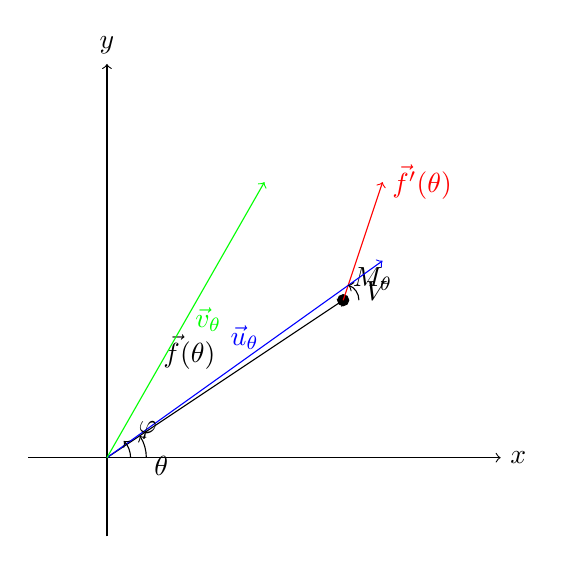
\begin{tikzpicture}
    % Axes
    \draw[->] (-1,0) -- (5,0) node[right] {$x$};
    \draw[->] (0,-1) -- (0,5) node[above] {$y$};
    
    % Point Mt
    \coordinate (Mt) at (3,2);
    \draw[fill] (Mt) circle [radius=2pt] node[above right] {$M_\theta$};
    
    % Vectors
    \draw[->] (0,0) -- (Mt) node[midway, above left] {$\vec{f}(\theta)$};
    \draw[->, red] (Mt) -- ++(0.5,1.5) node[right] {$\vec{f}'(\theta)$};
    \draw[->, blue] (0,0) -- (3.5,2.5) node[midway, above] {$\vec{u}_{\theta}$};
    \draw[->, green] (0,0) -- (2,3.5) node[midway, right] {$\vec{v}_{\theta}$};
    
    % Angles
    \draw[->] (0.5,0) arc [start angle=0, end angle=33.69, radius=0.5] node[midway, below right] {$\theta$};
    \draw[->] (Mt) ++(0.2,0) arc [start angle=0, end angle=71.57, radius=0.2] node[midway, right] {$V$};
    \draw[->] (0.3,0) arc [start angle=0, end angle=45, radius=0.3] node[midway, above right] {$\varphi$};
\end{tikzpicture}
\end{center}


 On calcule les limites de  $\rho$  aux bornes de son domaine de définition. Si  $\rho$  est dérivable, on calcule sa dérivée et on étudie son signe là où elle existe pour connaître les variations de  $\rho$ . On dispose enfin ces informations dans un tableau de variations :
%
%
%
% \item  la premi`ere ligne est celle contenant les valeurs permises de θ,
% \item  la seconde contient le signe de  \rho ′(θ),
% \item  la troisi`eme donne les valeurs, les variations et les limites de  \rho (θ).
%REMARQUE 6.11 :
% \item  Avec ce type de paramétrage, pour qu'un point soit stationnaire, il faut que  \rho (θ) =  \rho ′(θ) = 0 donc
%seul l'origine O du rep`ere peut ˆetre un point stationnaire.
% \item  De plus, lorsque lim
%θ→θ0
% \rho (θ) = 0, donc quand on passe au pˆole, on a aussi lim
%θ→θ0
%−−−→
%OMθ
%OMθ
%= ±−−→uθ0 donc le
%passage au pˆole s'effectue toujours selon le vecteur −−→uθ0 .



\subsection{Domaine d'étude et tableau de variations}


Comme pour une courbe en coordonnées cartésiennes, on détermine d'abord l'ensemble des $\theta$ possibles, c'est-à-dire le domaine de définition de la fonction $\rho$.

Ensuite on essaie de réduire ce domaine à un domaine d'étude plus petit mais qui contient les informations relatives à la courbe entière.\\

% \begin{Rmq}
\begin{itemize}
    \item Si $\rho$ est $2\pi$-périodique alors on peut étudier la courbe sur $D_f \cap [0; 2\pi]$ ou $D_f \cap [-\pi; \pi]$ et on repassera une infinité de fois par chacun des points de la courbe.\\
    
    \item Si $\rho$ est $\pi$-périodique on peut étudier et tracer la courbe sur $D_f \cap [0; \pi]$ ou $D_f \cap \left[ - \frac{\pi}{2}; \frac{\pi}{2} \right]$ et on obtiendra toute la courbe en effectuant une symétrie de centre $O$.\\
    
    \item Si $\rho$ est $T$-périodique en général, on peut étudier et tracer la courbe sur $D_f \cap [0; T]$ et on obtiendra ensuite toute la courbe par une infinité de rotations d'angle $T$.\\
    \item Si $\rho$ est paire alors on peut étudier et tracer la courbe sur $D_f \cap \mathbb{R}^+$ et on obtiendra ensuite toute la courbe ar une symétrie d'axe $(Ox)$.\\
    
    \item Si $\rho$ est impaire alors on peut étudier et tracer la courbe sur $D_f \cap \mathbb{R}^+$ et on obtiendra ensuite toute la courbe par une symétrie d'axe $(Oy)$.\\
    
    \item Si $\forall \theta \in D_f, \rho(\pi - \theta) = \rho(\theta)$ alors on peut étudier et tracer la courbe sur $Df \cap \left[ - \infty; \frac{\pi}{2} \right]$ et on obtiendra ensuite toute la courbe par une symétrie d'axe $(Oy)$.\\
    
    \item Si $\forall \theta \in D_f, \rho(\pi - \theta) = -\rho(\theta)$ alors on peut étudier et tracer la courbe sur $D_f \cap \left[ - \infty; \frac{\pi}{2} \right]$ et on obtiendra ensuite toute la courbe par une symétrie d'axe $(Ox)$.\\
    
    \item Si $\forall \theta \in D_f, \rho \left(\frac{\pi}{2} - \theta \right) = \rho(\theta)$ alors on peut étudier et tracer la courbe sur $D_f \cap \left[ - \infty; \frac{\pi}{2} \right]$ et on obtiendra ensuite toute la courbe par une symétrie d'axe $(Ox)$.\\
\end{itemize}
% \end{Rmq}

\subsection{Branches infinies et point multiples}

% \begin{Rmq} 
On a la même définition d'une branche infinie quand $\theta$ tend vers $\theta_0$ qu'en cartésiennes,
il faut que $\lim_{\theta \to \theta_0} |\rho(\theta)| = +\infty$, si c'est le cas on se place dans le nouveau repère $(O, \vec{u}_{\theta_0}, \vec{v}_{\theta_0})$ dans lequel le point $M_{\theta}$ admet pour coordonnées cartésiennes $(X, Y)$ avec :
\[
X = \rho(\theta) \cos(\theta - \theta_0) \quad \text{et} \quad Y = \rho(\theta) \sin(\theta - \theta_0).
\]

On a bien sûr $X \to \pm\infty$ lorsque $\theta \to \theta_0$. Par contre :


\begin{itemize}
 \item  si $Y$ n'a pas de limite en $\theta_0$ et on dit juste que la courbe admet pour direction asymptotique $\theta = \theta_0$.
 \item  si $\underset{\theta \to \theta_0}{\lim}Y = +\infty$
 on dit que la courbe admet une branche parabolique de direction $\theta = \theta_0$.
 \item  si $\underset{\theta \to \theta_0}{\lim}Y = Y_0$ la courbe admet une droite asymptote d'équation $Y = Y_0$ dans ce nouveau repère.\\
 \end{itemize}
 % \end{Rmq}
 
\begin{Def} \textbf{Point multiple}\\
Un point de la courbe est dit multiple s'il est associé à deux paramètres différents
(mais pas issu de la périodicité) sachant que, pour un point $M$ on a :

\[
M = M_{\theta_1} = M_{\theta_2} \Longleftrightarrow
\Big(
(\theta_1 \equiv \theta_2[2\pi] \text{ et }  \rho (\theta_1) =  \rho (\theta_2)\Big) 
\]
\[\text{ ou } \Big(\theta_1 \equiv \theta_2 + \pi[2\pi] \text{ et }   \rho (\theta_1) = - \rho (\theta_2)\Big)
)
\]

\end{Def}

\begin{Meth}\textbf{Pour étudier une courbe donnée en polaires par $\rho = \rho(\theta) $}\\

\begin{itemize}
 \item  On détermine d'abord le domaine de définition de la courbe.
 \item  On cherche aussi le plus petit domaine d'étude possible grâce aux propriétés de  $\rho$  et
on écrit les transformations géométriques qui permettent de retrouver ensuite toute la
courbe.
 \item  On calcule la dérivée de  $\rho$  et on dresse le tableau de variations global.
 \item  On étudie les branches infinies : asymptotes et position locale par rapport à celles-ci.
 \item  On trace la courbe en indiquant le sens de parcours et en positionnant les points à
tangentes orthoradiales, les passages au pôle, les croisements avec les axes, ....
 \item  Si on voit apparaître des points multiples, on essaie de les calculer.
\end{itemize}
\end{Meth}



\section{Exercices}

\exo[2]{Du tableau de variations à la courbe}
Soit $f:[0,+\infty[\to\mathbb R^2$ un arc paramétré de classe $C^1$, dont le tableau de variations des fonctions coordonnées
est :
$$
\begin{tabvar}{|C|CCCCCCCCC|} \hline 
t	&0 &  &&1	& & &\sqrt 3	& & +\infty
\\ \hline 
x'(t)  & 0	    &+ &&\dbarre& & + & & + &\\ \hline
 \niveau{1}{3} x(t) &1	&\croit
&\niveau{3}{3}+\infty&\dbarre	&\niveau{1}{3}-\infty&\croit &-\frac 12 &\croit& \niveau{3}{3}0 \\ \hline
  \niveau{1}{3} y(t) &0 &\croit & +\infty & \dbarre & \niveau{1}{3} -\infty & \croit &-\frac{3\sqrt 3}2 &\decroit&-\infty  \\ \hline 
  y'(t) &  0	    &+ &&\dbarre& & + &0 & -&\\ \hline 
\end{tabvar}
$$
Que peut-on dire, à la lecture de ce tableau, des points stationnaires? des tangentes parallèles aux axes? des branches infinies?\\
Tracer une courbe paramétrée qui peut correspondre à ce tableau de variations.\\
\vspace{1em}
\hrule
\vspace{1em}


% Exercice 1183

        
\newpage


\exo[2]{Branches infinies}


\'Etudier les branches infinies de la courbe paramétrée $t\mapsto \left(\frac{t^3}{t^2-9},\frac{t(t-2)}{t-3}\right).$\\
\vspace{1em}
\hrule
\vspace{1em}

% Exercice 1184


\exo [2]{ Recherche de point double}


Démontrer que la courbe paramétrée $t\mapsto \left(\displaystyle 2t-\frac 1{t^2},2t+t^2\right)$ possède un point double dont on donnera les coordonnées.\\
\vspace{1em}
\hrule
\vspace{1em}

% Exercice 1185


\exo[2]{\'Equation cartésienne}


Déterminer une équation cartésienne de l'arc paramétré $t\mapsto \left(\frac t{1-t^4},\frac{t^3}{1-t^4}\right)$.\\

\vspace{1em}
\hrule
\vspace{1em}
% Exercice 2540


\exo[3]{Tangente en un point stationnaire}


Pour $t\in \mathbb R\backslash\{-1,1\}$, on note $f(t)=\frac{t^2}{1-t^2}$ et $g(t)=\frac{t^3}{1-t^2}$. Dans un plan muni d'un repère $(O,\vec i,\vec j)$, on note $M(t)$ le point de coordonnées $(f(t),g(t))$ et $\mathcal C$ la courbe paramétrée $\{M(t);\ t\in \mathbb R\backslash\{-1,1\}\}$.
\begin{enumerate}
\item Rappeler sans justification le développement limité en 0 à l'ordre $1$ de $\frac{1}{1-u}$. 
\item Déterminer les développements limités des fonctions $f$ et $g$ à l'ordre $3$ en $0$.
\item En déduire la valeur de $f''(0)$ et celle de $g''(0)$.
\item Donner les coordonnées d'un vecteur tangent à $\mathcal C$ en $(0,0)=(f(0),g(0))$.
\end{enumerate}

\vspace{1em}
\hrule
\vspace{1em}
% Exercice 1189


\exo[1]{Astroïde}

Tracer la courbe paramétrée d'équation $t\mapsto (\cos^3 t,\sin^3 t)$.

\vspace{1em}
\hrule
\vspace{1em}
% Exercice 1190


\exo[2]{Lemniscate de Bernoulli}


On considère la courbe paramétrée 
$$t\mapsto \left(\frac{t}{1+t^4},\frac{t^3}{1+t^4}\right).$$
\begin{enumerate}
\item Que déduit-on du changement de variables $t\mapsto 1/t$? Sur quel intervalle peut-on réduire l'étude?
\item Construire la courbe.
\end{enumerate}
\vspace{1em}
\hrule
\vspace{1em}

% Exercice 1196

        
\newpage


\exo[3]{Branches infinies et point singulier}

\'Etudier la courbe paramétrée suivante : $t\mapsto \left(t+\frac 1t,t+\frac 1{2t^2}\right)$, $t\in\mathbb R^*$.
On étudiera en particulier la position par rapport aux asymptotes, et la tangente aux points stationnaires.

\vspace{1em}
\hrule
\vspace{1em}

% Exercice 2175


\exo[2]{La rosace à huit feuilles}

Construire la rosace d'équation polaire $\rho(\theta)=\sin(4\theta)$.
On fera notamment attention à se restreindre à l'intervalle d'étude le plus petit possible.

\vspace{1em}
\hrule
\vspace{1em}

% Exercice 2176


\exo[3]{Une boucle}

On considère la courbe d'équation polaire $\rho(\theta)=4\cos\theta-\frac 1{\cos\theta}$. 
\begin{enumerate}
\item Démontrer qu'on peut limiter l'intervalle d'étude à $[0,\pi/2[$.
\item \'Etudier la branche infinie de la courbe sur l'intervalle $[0,\pi/2[$.
\item Tracer la courbe, on précisera en particulier la tangente à la courbe aux points correspondant à $\theta=0$ et $\theta=\frac{\pi}{3}$.
\end{enumerate}

\vspace{1em}
\hrule
\vspace{1em}

% Exercice 2177


\exo[3]{Détaillée}

On considère la courbe paramétrée $\Gamma$ d'équation polaire $\rho(\theta)=1+\tan\theta$.
\begin{enumerate}
\item \'Etudier les symétries de $\Gamma$ et restreindre l'intervalle d'étude.
\item \'Etudier les variations de $\rho$.
\item Déterminer les asymptotes de $\Gamma$ (on en donnera une équation dans le répère initial).
\item Déterminer la (les) tangente(s) de la courbe en $O$.
\item Tracer (le support de) $\Gamma$.
\end{enumerate}

\vspace{1em}
\hrule
\vspace{1em}
% Exercice 2178


\exo[2]{Deux branches infinies}

\'Etudier et tracer la courbe paramétrée d'équation $\rho(\theta)=1+\frac{\frac{\pi}{4}}{\frac{\theta-\pi}{3}}$.


\vspace{1em}
\hrule
\vspace{1em}
\exo[2]{Longueur d'un arche de cycloïde}

Calculer la longueur d'une arche de cycloïde :
$$\left\{
\begin{array}{rcl}
x(t)=a(t-\sin t)\\
y(t)=a(1-\cos t)\\
\end{array}\right.$$
avec $0\leq t\leq 2\pi$.

\vspace{1em}
\hrule
\vspace{1em}
% Exercice 1940

        
\newpage


\exo[2]{Longueur d'une spire d'hélice}

Calculer la longueur d'une spire d'hélice circulaire :
$$\left\{
\begin{array}{rcl}
x(t)&=&a\cos t\\
y(t)&=&a\sin t\\
z(t)&=&ht
\end{array}\right.$$
avec $0\leq t\leq 2\pi$.
